

\tikzset{every picture/.style={line width=0.75pt}} %set default line width to 0.75pt

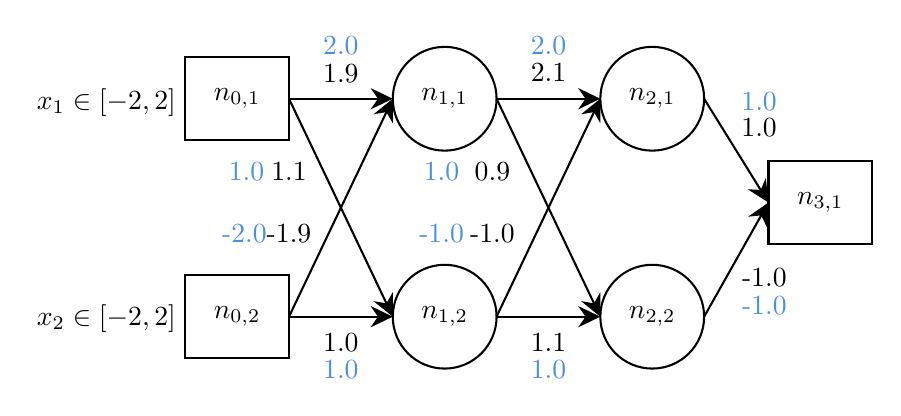
\begin{tikzpicture}[x=0.75pt,y=0.75pt,yscale=-1,xscale=1]
%uncomment if require: \path (0,395); %set diagram left start at 0, and has height of 395

%Shape: Circle [id:dp29452950296941915]
%\draw   (90,55) .. controls (90,41.19) and (101.19,30) .. (115,30) .. controls (128.81,30) and (140,41.19) .. (140,55) .. controls (140,68.81) and (128.81,80) .. (115,80) .. controls (101.19,80) and (90,68.81) .. (90,55) -- cycle ;
\draw (115,55) +(-25,-20) rectangle +(25,20) ;
%Shape: Circle [id:dp7730288688046164]
%\draw   (90,160) .. controls (90,146.19) and (101.19,135) .. (115,135) .. controls (128.81,135) and (140,146.19) .. (140,160) .. controls (140,173.81) and (128.81,185) .. (115,185) .. controls (101.19,185) and (90,173.81) .. (90,160) -- cycle ;
\draw (115,160) +(-25,-20) rectangle +(25,20) ;
%Shape: Circle [id:dp7848793538270885]
\draw   (190,160) .. controls (190,146.19) and (201.19,135) .. (215,135) .. controls (228.81,135) and (240,146.19) .. (240,160) .. controls (240,173.81) and (228.81,185) .. (215,185) .. controls (201.19,185) and (190,173.81) .. (190,160) -- cycle ;
%Shape: Circle [id:dp2581761932666119]
\draw   (190,55) .. controls (190,41.19) and (201.19,30) .. (215,30) .. controls (228.81,30) and (240,41.19) .. (240,55) .. controls (240,68.81) and (228.81,80) .. (215,80) .. controls (201.19,80) and (190,68.81) .. (190,55) -- cycle ;
%Shape: Circle [id:dp03162623697960232]
\draw   (290,160) .. controls (290,146.19) and (301.19,135) .. (315,135) .. controls (328.81,135) and (340,146.19) .. (340,160) .. controls (340,173.81) and (328.81,185) .. (315,185) .. controls (301.19,185) and (290,173.81) .. (290,160) -- cycle ;
%Shape: Circle [id:dp02546394024001375]
\draw   (290,55) .. controls (290,41.19) and (301.19,30) .. (315,30) .. controls (328.81,30) and (340,41.19) .. (340,55) .. controls (340,68.81) and (328.81,80) .. (315,80) .. controls (301.19,80) and (290,68.81) .. (290,55) -- cycle ;
%Shape: Circle [id:dp12084775666404268]
%\draw   (371,105) .. controls (371,91.19) and (382.19,80) .. (396,80) .. controls (409.81,80) and (421,91.19) .. (421,105) .. controls (421,118.81) and (409.81,130) .. (396,130) .. controls (382.19,130) and (371,118.81) .. (371,105) -- cycle ;
\draw (396,105) +(-25,-20) rectangle +(25,20) ;
%Straight Lines [id:da34998381745971496]
\draw    (140,160) -- (187,160) ;
\draw [shift={(190,160)}, rotate = 180] [fill={rgb, 255:red, 0; green, 0; blue, 0 }  ][line width=0.08]  [draw opacity=0] (10.72,-5.15) -- (0,0) -- (10.72,5.15) -- (7.12,0) -- cycle    ;
%Straight Lines [id:da4638805061238097]
\draw    (140,160) -- (188.71,57.71) ;
\draw [shift={(190,55)}, rotate = 475.46] [fill={rgb, 255:red, 0; green, 0; blue, 0 }  ][line width=0.08]  [draw opacity=0] (10.72,-5.15) -- (0,0) -- (10.72,5.15) -- (7.12,0) -- cycle    ;
%Straight Lines [id:da15742477491714235]
\draw    (140,55) -- (187,55) ;
\draw [shift={(190,55)}, rotate = 180] [fill={rgb, 255:red, 0; green, 0; blue, 0 }  ][line width=0.08]  [draw opacity=0] (10.72,-5.15) -- (0,0) -- (10.72,5.15) -- (7.12,0) -- cycle    ;
%Straight Lines [id:da9054930639679811]
\draw    (140,55) -- (188.71,157.29) ;
\draw [shift={(190,160)}, rotate = 244.54000000000002] [fill={rgb, 255:red, 0; green, 0; blue, 0 }  ][line width=0.08]  [draw opacity=0] (10.72,-5.15) -- (0,0) -- (10.72,5.15) -- (7.12,0) -- cycle    ;
%Straight Lines [id:da0727882271401632]
\draw    (240,160) -- (288.71,57.71) ;
\draw [shift={(290,55)}, rotate = 475.46] [fill={rgb, 255:red, 0; green, 0; blue, 0 }  ][line width=0.08]  [draw opacity=0] (10.72,-5.15) -- (0,0) -- (10.72,5.15) -- (7.12,0) -- cycle    ;
%Straight Lines [id:da02068180741540726]
\draw    (240,55) -- (288.71,157.29) ;
\draw [shift={(290,160)}, rotate = 244.54000000000002] [fill={rgb, 255:red, 0; green, 0; blue, 0 }  ][line width=0.08]  [draw opacity=0] (10.72,-5.15) -- (0,0) -- (10.72,5.15) -- (7.12,0) -- cycle    ;
%Straight Lines [id:da4941096166166473]
\draw    (340,55) -- (369.42,102.45) ;
\draw [shift={(371,105)}, rotate = 238.2] [fill={rgb, 255:red, 0; green, 0; blue, 0 }  ][line width=0.08]  [draw opacity=0] (10.72,-5.15) -- (0,0) -- (10.72,5.15) -- (7.12,0) -- cycle    ;
%Straight Lines [id:da0005753242144755921]
\draw    (340,160) -- (369.53,107.61) ;
\draw [shift={(371,105)}, rotate = 479.41] [fill={rgb, 255:red, 0; green, 0; blue, 0 }  ][line width=0.08]  [draw opacity=0] (10.72,-5.15) -- (0,0) -- (10.72,5.15) -- (7.12,0) -- cycle    ;
%Straight Lines [id:da6663993224468625]
\draw    (240,160) -- (287,160) ;
\draw [shift={(290,160)}, rotate = 180] [fill={rgb, 255:red, 0; green, 0; blue, 0 }  ][line width=0.08]  [draw opacity=0] (10.72,-5.15) -- (0,0) -- (10.72,5.15) -- (7.12,0) -- cycle    ;
%Straight Lines [id:da971612493075633]
\draw    (240,55) -- (287,55) ;
\draw [shift={(290,55)}, rotate = 180] [fill={rgb, 255:red, 0; green, 0; blue, 0 }  ][line width=0.08]  [draw opacity=0] (10.72,-5.15) -- (0,0) -- (10.72,5.15) -- (7.12,0) -- cycle    ;

% Text Node
\draw (165,43) node  [font=\normalsize] [align=left] {1.9};
% Text Node
\draw (140,90) node  [font=\normalsize] [align=left] {1.1};
% Text Node
\draw (140,120) node  [font=\normalsize] [align=left] {\mbox{-}1.9};
% Text Node
\draw (165,172.5) node  [font=\normalsize] [align=left] {1.0};
% Text Node
\draw (265,42.5) node  [font=\normalsize] [align=left] {2.1};
% Text Node
\draw (238,90) node  [font=\normalsize] [align=left] {0.9};
% Text Node
\draw (265,172.5) node  [font=\normalsize] [align=left] {1.1};
% Text Node
\draw (238,120) node  [font=\normalsize] [align=left] {\mbox{-}1.0};
% Text Node
\draw (366.5,69) node  [font=\normalsize] [align=left] {1.0};
% Text Node
\draw (369,141) node  [font=\normalsize] [align=left] {\mbox{-}1.0};
% Text Node
\draw (115,55) node  {$n_{0,1}$};
% Text Node
\draw (115,160) node    {$n_{0,2}$};
% Text Node
\draw (215,160) node    {$n_{1,2}$};
% Text Node
\draw (215,55) node    {$n_{1,1}$};
% Text Node
\draw (315,55) node    {$n_{2,1}$};
% Text Node
\draw (315,160) node    {$n_{2,2}$};
% Text Node
\draw (396,105) node    {$n_{3,1}$};
% Text Node
\draw (52,57) node    {$x_{1} \in [ -2,2]$};
% Text Node
\draw (52,161) node    {$x_{2} \in [ -2,2]$};
% Text Node
\draw (118.5,120) node  [font=\normalsize,color={rgb, 255:red, 74; green, 144; blue, 226 }  ,opacity=1 ] [align=left] {\mbox{-}2.0};
% Text Node
\draw (119.5,90) node  [font=\normalsize,color={rgb, 255:red, 74; green, 144; blue, 226 }  ,opacity=1 ] [align=left] {1.0};
% Text Node
\draw (165,29.5) node  [font=\normalsize,color={rgb, 255:red, 74; green, 144; blue, 226 }  ,opacity=1 ] [align=left] {2.0};
% Text Node
\draw (165,185.5) node  [font=\normalsize,color={rgb, 255:red, 74; green, 144; blue, 226 }  ,opacity=1 ] [align=left] {1.0};
% Text Node
\draw (213.5,120) node  [font=\normalsize,color={rgb, 255:red, 74; green, 144; blue, 226 }  ,opacity=1 ] [align=left] {\mbox{-}1.0};
% Text Node
\draw (213.5,90) node  [font=\normalsize,color={rgb, 255:red, 74; green, 144; blue, 226 }  ,opacity=1 ] [align=left] {1.0};
% Text Node
\draw (265,29.5) node  [font=\normalsize,color={rgb, 255:red, 74; green, 144; blue, 226 }  ,opacity=1 ] [align=left] {2.0};
% Text Node
\draw (265,185.5) node  [font=\normalsize,color={rgb, 255:red, 74; green, 144; blue, 226 }  ,opacity=1 ] [align=left] {1.0};
% Text Node
\draw (366.5,56.5) node  [font=\normalsize,color={rgb, 255:red, 74; green, 144; blue, 226 }  ,opacity=1 ] [align=left] {1.0};
% Text Node
\draw (369,154.5) node  [font=\normalsize,color={rgb, 255:red, 74; green, 144; blue, 226 }  ,opacity=1 ] [align=left] {\mbox{-}1.0};


\end{tikzpicture}
